\documentclass{article}
\usepackage[utf8]{inputenc}
\usepackage{graphicx} %package to manage images
\graphicspath{ {./images/} }

\usepackage[rightcaption]{sidecap}

\usepackage{wrapfig}

\title{Link prediction based on local random walk}
\author{Itwinder Singh}
\date{}

\begin{document}

\maketitle
        
\section{Introduction}
The process of predicting missing links in complex networks has gained significant interest of late. It calculates the probability of a link between two nodes. In particular networks, for example biological networks the current knowledge is incomplete and results in expensive, in field or in laboratory, link discoveries. An efficient and cost effective way is to accurately predict the existence of links based on observed links and narrow down those which are most likely to be present instead of scoping all possible links. In social friendship networks, it can guide the users to the possibility of a likely link which is currently non existent.\par
In general, similar nodes have more chance of being linked. Similarities can be based on essential node attributes or on the structure of network. Similarities indices can be of local type, based primarily on node degree and local neighborhood. Other similarity indices are path dependent and require global knowledge of network topology. Local indices are less complex and more efficient then global indices, however due to lack of sufficient data they have less prediction accuracy. The main challenge is to design and develop an efficient and accurate algorithm for link prediction.\par
\section{Method}
Local random walk (LWR) similarity index was used in this article because of it's less computational complexity compared to other random walk similarity indices. This method and other similarity indices(3 local,3 global) were used to evaluate 5 real networks and results compared.\par
A undirected simple network was chosen in which self connections and multiple links were not allowed. A similarity score was assigned to each pair of nodes. Real networks have high clustering coefficients while most random walk similarity measures have a small probability of a walker moving to a node further away in the network than to a close by node which results in low prediction accuracy. Superposed random walk (SRW) is used to counter that by releasing the walker from the same position and their contributions superposed. Observed links are randomly divided into training set and probe set. Standard metrices, AUC(Area under curve) and Precision were used to evaluate the accuracy of results. An AUC score closer to 1 shows the model has greater measure of separability while a score near 0 indicates poor separability. High precision reflects better prediction accuracy.\par 

\section{Results}
Plotted graphs and tables show that global indices are more accurate than local indices but LRW and SRW indices predictions are overall better in both AUC and precision. Their accuracy are not restricted to a particular density. LRW and SRW have shown to be more accurate and with less computational complexity can run calculations faster, though global indices generate more information besides just link prediction.

\section{Appendix}

Tables and Figures\par
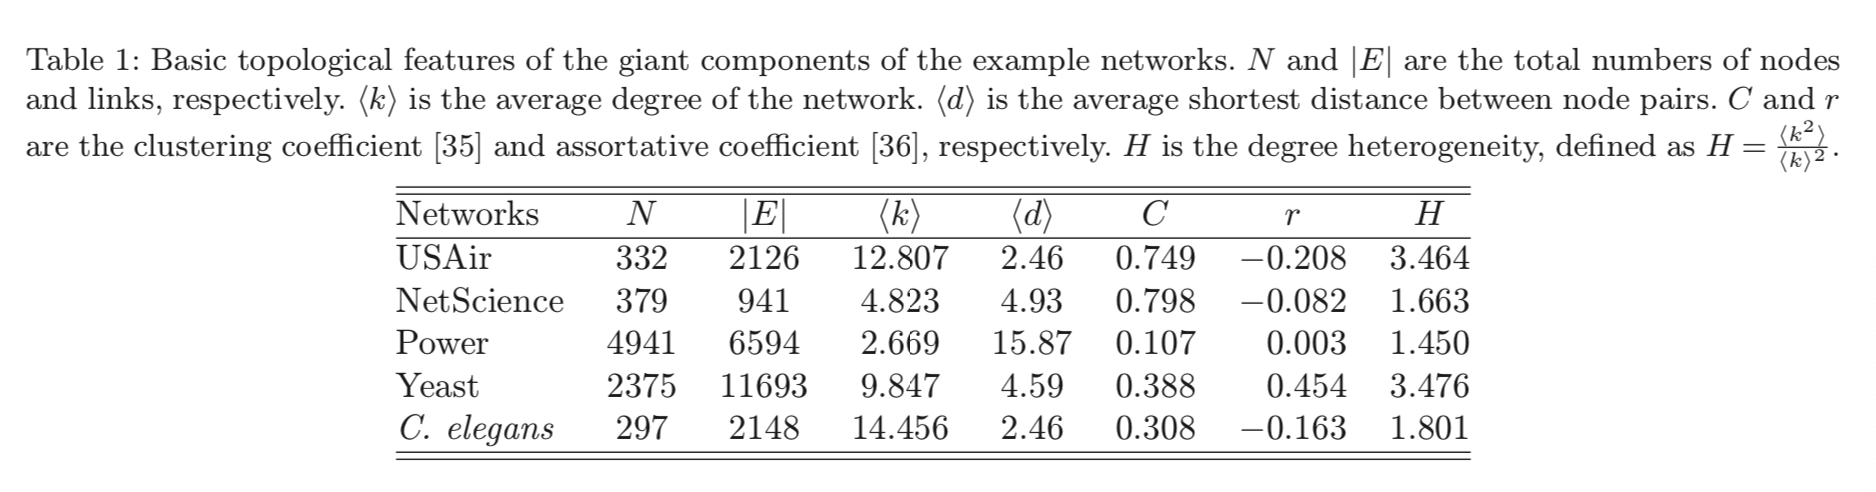
\includegraphics[scale=0.35]{images/Table1.png}\par
\\


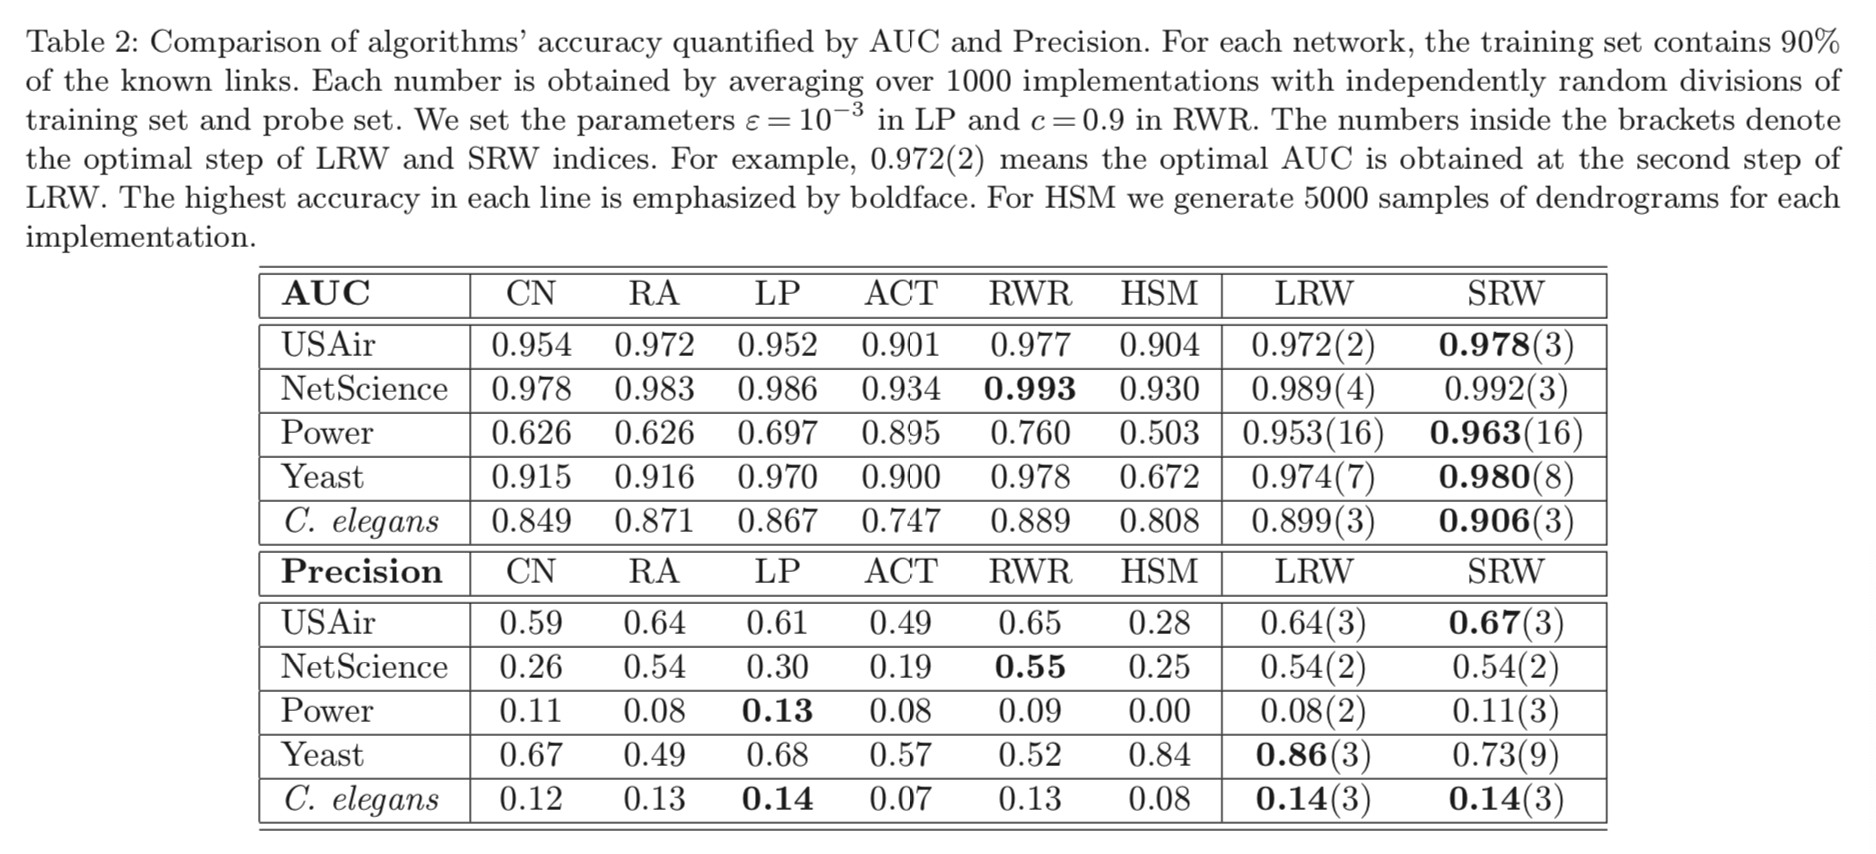
\includegraphics[scale=0.35]{images/Table2.png}

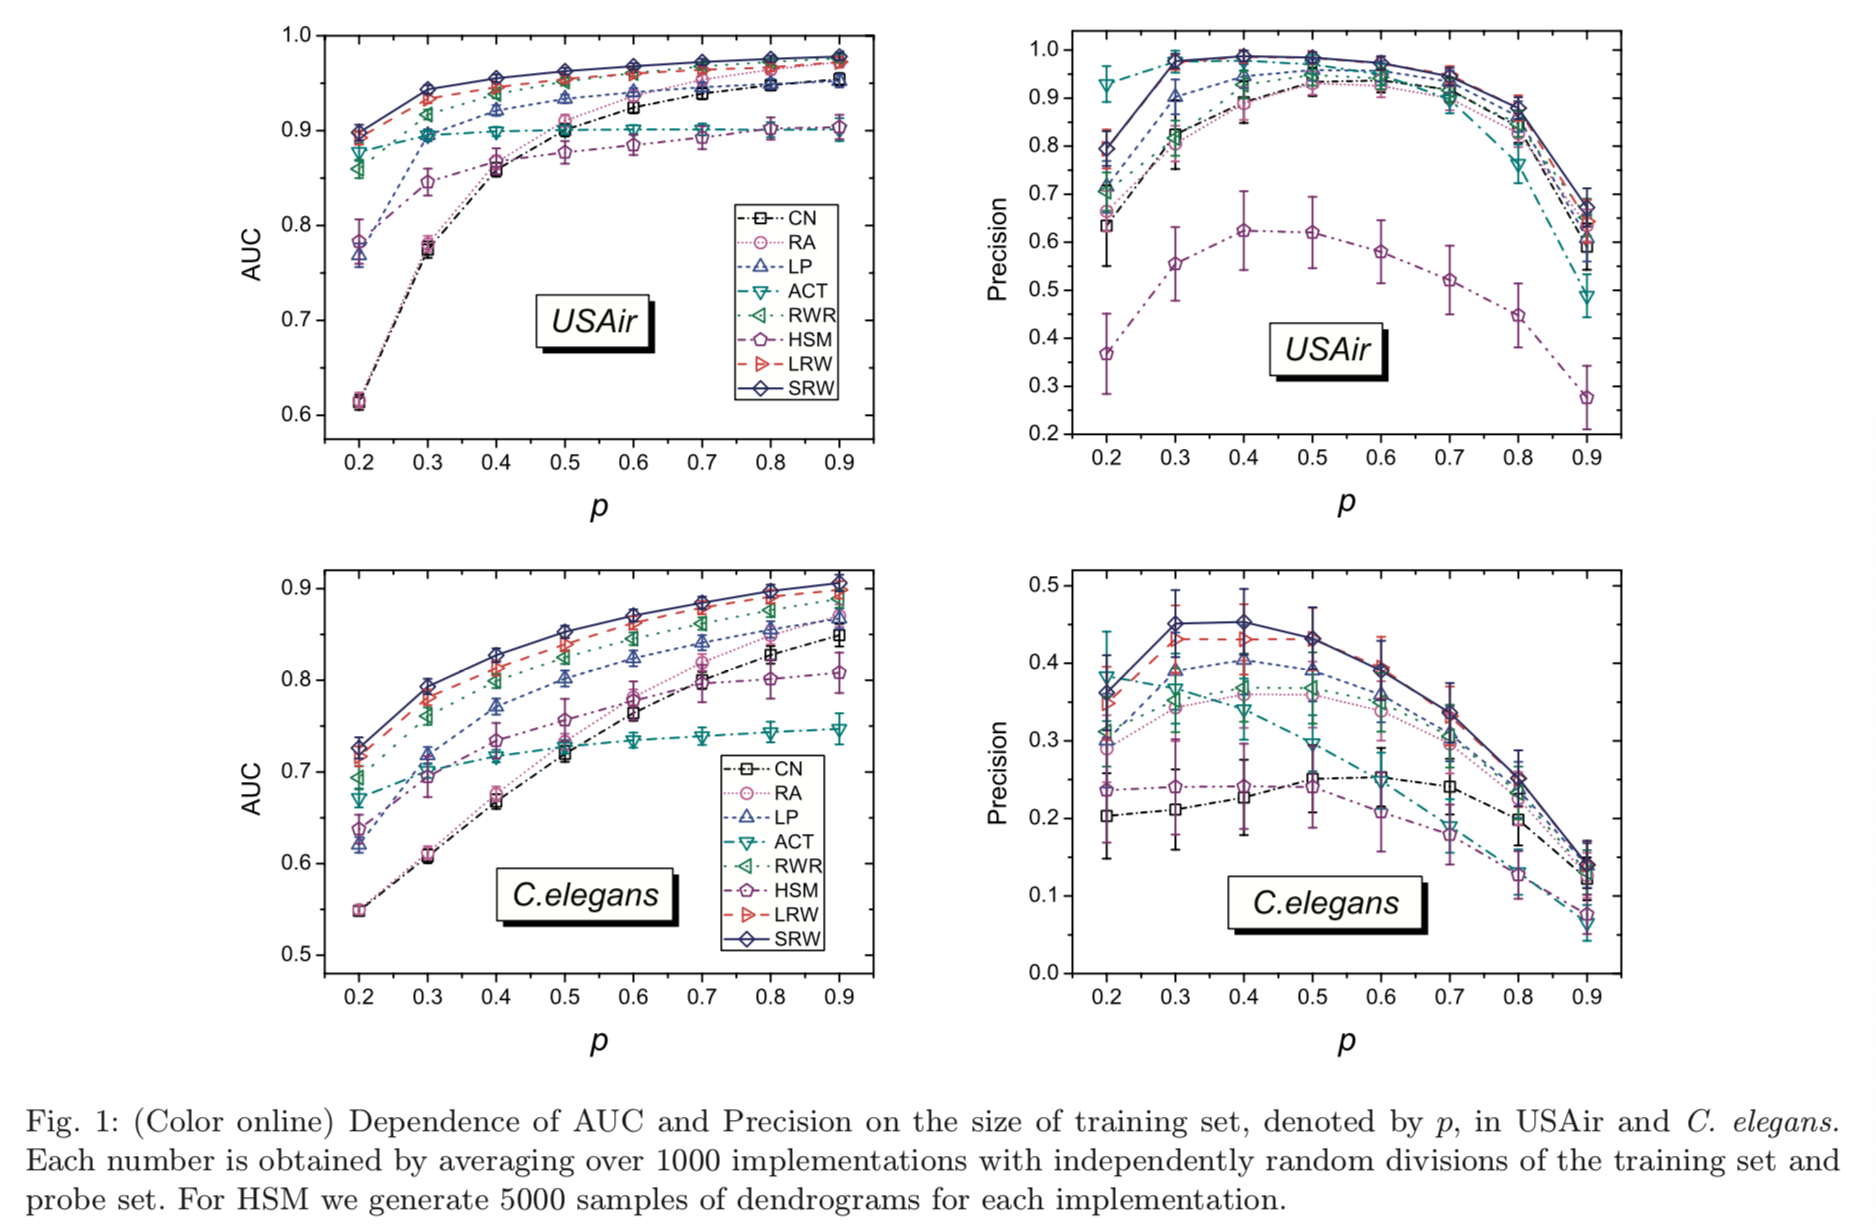
\includegraphics[scale=0.35]{images/Figure1.png}



\section{References}
1. Weiping Liu and Linyuan Lü 2010 EPL 89 58007











\end{document}


